\documentclass[10pt,a4paper]{article}
\usepackage{amsmath,amssymb,amsthm,graphicx}
\usepackage{amsmath,amssymb,amsthm,graphicx}
\usepackage{hyperref}
\newtheorem{theorem}{Theorem}
\newtheorem{definition}[theorem]{Definition}
\newtheorem{proposition}[theorem]{Proposition}
\newtheorem{lemma}[theorem]{Lemma}
\newtheorem{claim}[theorem]{Claim}
\newtheorem{remark}[theorem]{Remark}
\newcommand{\C}{\mathbb C}
\newcommand{\N}{\mathbb N}
\newcommand{\fcom}{f_{\rm com}}
\newcommand{\Gcom}{\Gamma_{\rm com}}
\newcommand{\g}{\mathfrak g}
\newcommand{\End}{\mathrm{End}}
\newcommand{\GL}{\mathrm{GL}}
\newcommand{\ncw}{\mathrm{ncw}}
\DeclareMathOperator{\linspan}{linspan}
\DeclareMathOperator{\im}{im}
\DeclareMathOperator{\inset}{in}
\DeclareMathOperator{\outset}{out}
\allowdisplaybreaks
\AtBeginDocument{\author{Markus Bl\"aser, Christian Ikenmeyer, Meena Mahajan\\Anurag Pandey, Nitin Saurabh}}
\title{Trace algebraic branching programs are not closed: an explicit degeneration separated by tangent-space flow dimensions}
\author{Markus Bläser, Christian Ikenmeyer, Meena Mahajan, Anurag Pandey, Nitin Saurabh}
\date{doi:10.4230/LIPIcs.CCC.2020.21; CC BY 3.0 Unported}
\begin{document}
\maketitle
\noindent\textit{Editorial note.} Editable transcription of complete formally published CCBY3.0Unported maintrace proof andnecessarycontext. Native retrieval timedout after boundedofficial attempts; no native version required or unpublished proof imported. FullSections5–8 retained, including author analogical-case statements, allsource-local flow/tangent arguments andfinalparityconstraint. Original author formulas, indices andconditions preserved withoutmathematicalrepair, newassumptions orreplacementproof. Onlydisplay wrapping/standardTeXglyph commands adapted. Underline denotesborderwidth as inpublication. ActualFigures1–3 extractedaslicenseddiagram crops, allproof prose/derivations editable. Originalnumbered bracketreferences keep complete42-entryordinarybibliography. SubsequentSection9 VQP/VNP discussion notselected orcounted. Allproduction/validationYupeng; rootownscompilation.\par\medskip
\noindent\textit{Allowed standard prerequisites (editorial).}\begin{itemize}
\item Complex tensor representations, flattening rank, orbit tangent spaces and classical graph-flow dimensions/cycle bases. Originalintro/Section3 conventions and completeSections5–8 definitions retained; standardflow rank/basis facts cited as[8], allsource-local construction anddimension proofs included
\end{itemize}\medskip
\section*{Models and border width (original Sections1 and3)}
An ABP is a layered directed graph with $d+1$ layers of vertices (edges only go from layers $i$ to $i+1$) such that the first and last layer have exactly the same number of vertices. Each vertex in the first layer has exactly one so-called corresponding vertex in the last layer. One interesting classical case is when the first and last layer have exactly one vertex, which is usually studied in theoretical computer science. We call this the single-(source,sink) model. Among algebraic geometers working on ABPs it is common to not impose restrictions on the number of vertices in the first and last layer. We call this the trace model. Every edge in an ABP is labeled by a homogeneous linear form. If we denote by $\ell(e)$ the homogeneous linear form of edge $e$, then we say that the ABP computes $\sum_p\prod_{e\in p}\ell(e)$, where the sum is over all paths that start in the first layer and end in the last layer at the vertex corresponding to the start vertex.
The width of an ABP is the number of vertices in its largest layer. We denote by $w(f)$ the minimal width required to compute $f$ in the trace model and we call $w(f)$ the trace ABP width complexity of $f$. We denote by $w_1(f)$ the minimal width required to compute $f$ in the single-(source,sink) model and we call $w_1(f)$ the single-(source,sink) ABP width complexity of $f$.
The border trace ABP width complexity $\underline w(f)$ is the smallest $w$ such that $f$ can be approximated arbitrarily closely by polynomials $f_\varepsilon$ with $w(f_\varepsilon)\le w$. Analogously, we define the border single-(source,sink) ABP width complexity $\underline w_1(f)$ as the smallest $w$ such that $f$ can be approximated arbitrarily closely by polynomials $f_\varepsilon$ with $w_1(f_\varepsilon)\le w$.
In the noncommutative homogeneous setting, $R_d=\mathbb F\langle x_1,\ldots,x_m\rangle_d$. We write $\ncw$ instead of $w$ and $\ncw_1$ instead of $w_1$ to highlight that we are in the noncommutative setting. The coefficient vectors identify this space with the $d$-th tensor power of $\mathbb F^m$. Over $\C$ the Zariski-closure of a set of polynomials of bounded complexity equals its Euclidean closure, by the standard principle cited in originalSection1.
For a homogeneous degree-$d$ ABP $\Gamma$, we denote by $V$ the set of vertices of $\Gamma$ and by $V^i$ the set of vertices in layer $i$, $1\le i\le d+1$. We choose an explicit bijection between the sets $V^1$ and $V^{d+1}$, so that each vertex $v$ in $V^1$ has exactly one corresponding vertex $\operatorname{corr}(v)$ in $V^{d+1}$. We denote by $E^i$ the set of edges from $V^i$ to $V^{i+1}$. Let $E$ denote the union of all $E^i$.
There is a classical interpretation in terms of iterated matrix multiplication: Fix some arbitrary ordering of the vertices within each layer, such that the $i$-th vertex in $V^1$ corresponds to the $i$-th vertex in $V^{d+1}$. For $1\le k\le d$ let $M_k$ be the $|V^k|\times|V^{k+1}|$ matrix whose entry at position $(i,j)$ in $M_k$ is the label from the $i$-th vertex in $V^k$ to the $j$-th vertex in $V^{k+1}$. Then $\Gamma$ computes the trace
\[\sum_{\substack{1\le k_1\le|V^1|\\1\le k_2\le|V^2|\\\cdots\\1\le k_d\le|V^d|}}(M_1)_{k_1,k_2}\cdots(M_{d-1})_{k_{d-1},k_d}(M_d)_{k_d,k_1}=\operatorname{tr}(M_1M_2\cdots M_d).\tag{8}\]
Hence the name trace model. In the single-(source,sink) model, the trace is taken of a $1\times1$ matrix.
\section*{5 Explicit construction of $f_0$ with higher complexity than border complexity}
Fix some $d\ge3$. In this section for every $m\ge2$ we construct $f_0$ such that
\[m=\underline{\ncw}(f_0)<\ncw(f_0).\tag{10}\]
A completely analogous construction can be used to find $f_0$ with $\underline w(f_0)<w(f_0)$ and with $\underline{\mathrm{mw}}(f_0)<\mathrm{mw}(f_0)$. For the sake of simplicity, we carry out only the proof for (10).
Recall that in a format $w$ ABP we have $w_{d+1}=w_1$. In each layer $i$ we enumerate the vertices $V^i=\{v^i_1,\ldots,v^i_{w_i}\}$ and we assume without loss of generality that the correspondence bijection between $V^{d+1}$ and $V^1$ is the identity on the indices $j$ of $v^1_j$, i.e., the $j$th vertex in $V^1$ corresponds to the $j$th vertex in $V^{d+1}$.
Fix an ABP format $w=(w_1,w_2,\ldots,w_d)$ such that for all $i$, $w_i\ge2$. Let $\Gcom$ denote the directed acyclic graph underlying an ABP of format $w$. An edge can be described by the triple $(a,b,i)$, where $1\le i\le d$, $1\le a\le w_i$ and $1\le b\le w_{i+1}$. Consider the following labeling of the edges with triple-indexed variables: $\ell_{\rm com}((a,b,i))=x^{(i)}_{(a,b)}$. Define $\fcom$ to be the polynomial computed by $\Gcom$ with edge labels $\ell_{\rm com}$.
We now construct $f_0$ as follows. Let $d$ be odd (the case when $d$ is even works analogously). Since in each layer we enumerated the vertices, we can now assign to each vertex its parity: even or odd. We call an edge between two even or two odd vertices parity preserving, while we call the other edges parity changing. Let us consider the following labeling of $\Gcom$: We set $\ell_0((a,b,i)):=x^{(i)}_{(a,b)}$ if $(a,b,i)$ is parity changing (i.e., $a\not\equiv b\pmod2$) and set the label $\ell_0((a,b,i)):=\varepsilon x^{(i)}_{(a,b)}$ otherwise, where $\varepsilon\in\C$. Let $f'_\varepsilon$ be the polynomial computed by $\Gcom$ with edge labels $\ell_0$ and set $f_\varepsilon:=\frac1\varepsilon f'_\varepsilon$ for $\varepsilon\ne0$. We define $f_0:=\lim_{\varepsilon\to0}f_\varepsilon$ (convergence follows from the construction, because $d$ is odd). By definition, for all $\varepsilon\ne0$, $f_\varepsilon$ can be computed by a format $w$ ABP. However, we will now prove that this property fails for the limit point $f_0$.
\setcounter{theorem}{3}

\begin{theorem}\label{thm:nonclosure}
Fix an ABP format $w=(w_1,w_2,\ldots,w_d)$ such that for all $i$, $w_i\ge2$. Let $f_0$ be defined as above. Then, $f_0$ cannot be computed by an ABP of format $w$.
\end{theorem}

Note that for a format where $m=w_1=\cdots=w_d$, this gives the $f_0$ which was desired in (10). (Note, however, that $f_0$ can be computed by an ABP of width $2m$ as follows. Construct an ABP $\Gamma'$ that has, for each vertex $v\in\Gcom$, vertices $v'$ and $v''$. For each parity changing edge $(a,b)\in\Gcom$ with label $\ell_0$, add edges $(a',b')$ and $(a'',b'')$ with the same label $\ell_0$. For each parity preserving edge $(a,b)\in\Gcom$ with label $\ell_0$, add edge $(a',b'')$ with label $(\frac1\varepsilon)\ell_0$. For corresponding vertices $u,v$ in $\Gcom$, let $v''$ be the corresponding vertex for $u'$ and $v'$ be the corresponding vertex for $u''$ in $\Gamma'$. All paths between corresponding vertices in this ABP use exactly one parity preserving edge of $\Gcom$, and so this ABP computes $f_0$.)
The proof of Theorem 4 works as follows. Let $G:=\GL_{w_1w_2}\times\GL_{w_2w_3}\times\cdots\times\GL_{w_dw_{d+1}}$. Let $\End:=\overline G$ denote its Euclidean closure, i.e., tuples of matrices in which one or several matrices can be singular.
We consider noncommutative homogeneous polynomials in the variables $x^{(i)}_{(a,b)}$ such that the $i$-th variable in each monomial is $x^{(i)}_{(a,b)}$ for some $a\in[w_i]$ and $b\in[w_{i+1}]$. The vector space of these polynomials is isomorphic to $W:=\C^{w_1w_2}\otimes\C^{w_2w_3}\otimes\cdots\otimes\C^{w_dw_{d+1}}$ and the monoid $\End$ (and thus also the group $G$) acts on this space in the canonical way. The set
\[\{f\in W\mid f\text{ can be computed by a format }w\text{ ABP}\}\]
is precisely the orbit $\End\fcom$. We follow the overall proof strategy in [24]. The monoid orbit $\End\fcom$ decomposes into two disjoint orbits:
\[\End\fcom=G\fcom\cup(\End\setminus G)\fcom.\]
Our goal is to show two things independently:
\begin{enumerate}\item $f_0\notin(\End\setminus G)\fcom$, and\item $f_0\notin G\fcom$,\end{enumerate}
which finishes the proof of Theorem 4.
All elements in $(\End\setminus G)\fcom$ are not concise, a term that we define in Section 6, where we also prove that $f_0$ is concise. Therefore $f_0\notin(\End\setminus G)\fcom$.
All elements in $G\fcom$ have full orbit dimension, a term that we define in Section 7 and we prove that $f_0$ does not have full orbit dimension in Section 8. This finishes the proof of Theorem 4.

\section*{6 Conciseness}
In this section we show that $f_0\notin(\End\setminus G)\fcom$. To do so we use a notion called conciseness. Informally, it captures whether a polynomial depends on all variables independent of a change of basis, or a tensor cannot be embedded into a tensor product of smaller spaces.
Given a tensor $f$ in $\C^{m_1}\otimes\C^{m_2}\otimes\cdots\otimes\C^{m_d}$, we associate the following matrices with $f$. For $j\in[d]$, define a matrix $M_f^j$ of dimension $m_j\times(\prod_{i\in[d]\setminus\{j\}}m_i)$ with rows labeled by the standard basis of $\C^{m_j}$, and columns by elements in the Cartesian product
\begin{multline*}
\{\text{standard basis of }\C^{m_1}\}\times\cdots\times\{\text{standard basis of }\C^{m_{j-1}}\}\\
\times\{\text{standard basis of }\C^{m_{j+1}}\}\times\cdots\times\{\text{standard basis of }\C^{m_d}\}.
\end{multline*}
We write the tensor $f$ in the standard basis
\[f=\sum_{\substack{1\le i_1\le m_1\\1\le i_2\le m_2\\\cdots\\1\le i_d\le m_d}}\alpha_{i_1,\ldots,i_d}e_{i_1}\otimes\cdots\otimes e_{i_d}\]
and associate to it the matrix $M_f^j$ whose entry at position $((i_j),(i_1,i_2,\ldots,i_{j-1},i_{j+1},\ldots,i_d))$ is $\alpha_{i_1,\ldots,i_d}$.
\begin{definition}
We say that a tensor $f$ in $\C^{m_1}\otimes\C^{m_2}\otimes\cdots\otimes\C^{m_d}$ is concise if and only if for all $j\in[d]$, $M_f^j$ has full rank.\footnote{When $f$ is viewed as a set-multilinear polynomial (see [36, Section 1.4]), this condition translates to the linear independence of the partial derivatives of $f$. In particular, $M_f^j$ is testing if the partial derivatives of $f$ with respect to the $j$-th block of variables are all linearly independent. This partial derivatives based criterion for testing if a polynomial depends on all the variables, independent of a change of basis, is pretty standard: see, for instance, [23, Corollary5.1.4].}
\end{definition}
As a warm-up exercise we now show that $\fcom$ is concise.
\begin{proposition}$\fcom$ is concise.\end{proposition}
\begin{proof}
We know that $\fcom\in W$. Let us consider the matrix $M^j_{\fcom}$ for some $j\in[d]$. To establish that $M^j_{\fcom}$ has full rank, it suffices to show that rows are linearly independent. In order to show that, we argue that every row is non-zero and every column has at most one non-zero entry. In other words, rows are supported on disjoint sets of columns.
A row of $M^j_{\fcom}$ is labeled by an edge in the $j$-th layer of the ABP $\Gcom$. Recall that only paths that start at a vertex in $V^1$ and end at the corresponding vertex in $V^{d+1}$ contribute to the computation in $\Gcom$. We call such paths valid paths. An entry in $M^j_{\fcom}$ is non-zero iff the corresponding row and column labels form a valid path in $\Gcom$. Thus, it is easily seen that a row is non-zero iff there is a valid path in $\Gcom$ that passes through the edge given by the row label. By the structure of $\Gcom$, in particular that every layer is a complete bipartite graph, we observe that passing through every edge there is some valid path. Hence, we obtain that every row is non-zero.
The second claim now follows from the observation that fixing $d-1$ edges either defines a unique $d$th edge so that these $d$ edges form a valid path, or for these $d-1$ edges there is no such $d$th edge.
\end{proof}
As mentioned in Section 5, to establish $f_0\notin(\End\setminus G)\fcom$ we will show that $f_0$ is concise while any element in $(\End\setminus G)\fcom$ is not.
\begin{lemma}$f_0$ is concise.\end{lemma}
\begin{proof}
Analogous to the proof of Proposition 6, we again show that every row of $M^j_{f_0}$ is non-zero and every column of it has at most one non-zero entry. That is, rows of $M^j_{f_0}$ are supported on disjoint sets of columns.
From the construction of $f_0$ it is seen that a path in $\Gcom$ contributes to the computation of $f_0$ iff it is a valid path that comprises of exactly one parity preserving edge. The second claim of every column having at most one non-zero entry now follows for the same reason as in the proof of Proposition 6.
Before proving the first claim, we recall two assumptions in the construction of $f_0$. The first is that the format $w=(w_1,w_2,\ldots,w_d)$ is such that $w_i\ge2$ for all $i\in[d]$ and the second is that $d$ is odd. To argue that a row is non-zero it suffices to show that a valid path comprising of only one parity preserving edge passes through the edge given by the row level.
Let us consider an arbitrary edge $e$ in $\Gcom$. We have two cases to consider depending on whether it is parity preserving or changing.
\paragraph{Case1.} Suppose $e$ is parity preserving and it belongs to a layer $j\in[d]$. The number of layers on the left of $e$ is $j-1$ and on the right is $d-j$. Since $d$ is odd, these numbers are either both even or both odd. We now argue for the case when they are even (the odd case is analogous). Choose a vertex $v$ in $V^1$ that has the same parity (different in the odd case) as one of the end points of $e$. (Such a choice exists because $w_1\ge2$.) We now claim that there exists a valid path starting at $v$ that passes through $e$ and contains exactly one parity preserving edge. Since $e$ is parity preserving, all edges in the claimed path must be parity changing. We observe that $e$ can be easily extended in both directions using parity changing edges such that the path ends at $\operatorname{corr}(v)$. The existence of parity changing edges at each layer uses the assumption that $w_i\ge2$.
\paragraph{Case2.} Otherwise $e=(a,b)$ is parity changing. Again as before there are two cases based on whether both $j-1$ and $d-j$ are even or odd. Consider the case when they are even (the odd case being analogous). We first assume that $j\ne d$. Choose a vertex $v$ in $V^1$ that has the same parity as $a$. We now construct a valid path from $v$ to $\operatorname{corr}(v)$ that passes through $e$ and contains exactly one parity preserving edge. It is easily seen that there exists a path from $v$ to $a$ using only parity changing edges. We choose a parity preserving outgoing edge incident to $b$. We call its endpoint $v_1$. Since $v_1$ and $v$ have different parities, we can connect $v_1$ to $\operatorname{corr}(v)$ in $V^{d+1}$ using only parity changing edges. Thus we obtain the following valid path $v\to\cdots\to a\to b\to v_1\to\cdots\to\operatorname{corr}(v)$ passing through exactly one parity preserving edge $(b,v_1)$. In the case that $j=d$, choose an incoming parity preserving edge incident on $a$ instead of an outgoing edge on $b$.
\end{proof}
\begin{remark}
We note that if the format $w=(w_1,\ldots,w_d)$ defining $f_0$ is such that for some $j\in[d]$, $w_j=1$, then $f_0$ is not concise. This can be seen as follows.
Let $w_j=1$, and let $v$ denote the unique vertex in $V^j$. Let $e$ be the edge $e=(1,1,j)$. If $j<d$, let $e'$ be the edge $e'=(1,1,j+1)$, otherwise let $e'$ be the edge $e'=(1,1,j-1)$. Both $e,e'$ are parity preserving edges. By construction, every valid path using $e'$ must also use $e$. Hence the corresponding row in the matrix $M^{j+1}_{f_0}$ if $j<d$, and in $M^{j-1}_{f_0}$ otherwise, is zero. Therefore $f_0$ is not concise.
This is an interesting observation, because this is the point where our proof fails for single-(source,sink) ABPs, and this is expected, because Nisan [35] had shown that the set of polynomials computed by such ABPs of format $w$ is a closed set.
\end{remark}
\begin{lemma}Let $f\in(\End\setminus G)\fcom$. Then $f$ is not concise.\end{lemma}
\begin{proof}
This statement is true in very high generality. In our specific case a proof goes as follows. If $f\in(\End\setminus G)\fcom$, then $f=g\fcom$ for some $g\in\End\setminus G$. Let $g=(g_1,\ldots,g_d)$, where $g_i\in\C^{w_iw_{i+1}\times w_iw_{i+1}}$. Since $g\notin G$, at least one of the $g_i$ must be singular. The crucial property is $M^i_{g\fcom}=g_iM^i_{\fcom}$, which finishes the proof.
\end{proof}

\section*{7 Orbit dimension, tangent spaces, and flows}
In this section we introduce tangent spaces and study their dimensions. We especially study them in the context of $G\fcom$, and $Gf_0$.
The orbit dimension of a tensor $f\in\C^{w_1w_2}\otimes\C^{w_2w_3}\otimes\cdots\otimes\C^{w_dw_{d+1}}$ is the dimension of the orbit $Gf$ as an affine variety. It can be determined as the dimension of the tangent space $T_f$ of the action of $G$ at $f$, which is a vector space defined as follows. Let $\g:=\C^{w_1w_2\times w_1w_2}\times\cdots\times\C^{w_dw_{d+1}\times w_dw_{d+1}}$. For $A\in\g$ we define the Lie algebra action $Af:=\lim_{\varepsilon\to0}\frac1\varepsilon((\mathrm{id}+\varepsilon A)f-f)$, where $\mathrm{id}\in G$ is the identity element. We define the vector space $T_f:=\g f=\{Af\mid A\in\g\}$.
\begin{claim}The dimension $\dim T_h$ is the same for all $h\in Gf$.\end{claim}
\begin{proof}
Since the action of $G$ is linear, for all $g\in G$ and $A\in\g$ we have
\begin{align*}
A(gf)&=\lim_{\varepsilon\to0}\frac1\varepsilon((\mathrm{id}+\varepsilon A)(gf)-gf)\\
&=\lim_{\varepsilon\to0}\frac1\varepsilon(gg^{-1}(\mathrm{id}+\varepsilon A)gf-gf)\\
&=g\lim_{\varepsilon\to0}\frac1\varepsilon((\mathrm{id}+\varepsilon(g^{-1}Ag))f-f)\\
&=g((g^{-1}Ag)f).
\end{align*}
Since $A\mapsto g^{-1}Ag$ is a bijection on $\g$, it follows that $T_{gf}=gT_f$. Hence the claim follows.
\end{proof}
In the following we will use Claim 10 to argue $f_0\notin G\fcom$ by showing that $\dim T_{\fcom}$ and $\dim T_{f_0}$ are different.
Let $e,e'\in E^i$ and let $A^{(i)}_{e,e'}\in\g$ denote the matrix tuple where the $i$-th matrix has a 1 at position $(e,e')$ and all other entries (also in all other matrices) are 0. Since these matrices form a basis of $\g$, it follows that
\[\g f=\linspan\{A^{(i)}_{e,e'}f\}.\]
For a tensor $f$ we define the support of $f$ as the set of monomials (i.e., standard basis tensors) for which $f$ has nonzero coefficient. For a linear subspace $V\subseteq\C^{w_1w_2}\otimes\C^{w_2w_3}\otimes\cdots\otimes\C^{w_dw_{d+1}}$ we define the support of $V$ as the union of the supports of all $f\in V$.
We write $e\cap e'=\varnothing$ to indicate that two edges $e$ and $e'$ do not share any vertex. We write $|e\cap e'|=1$ if they share exactly one vertex. We observe that for $f\in\{\fcom,f_0\}$ the vector space $T_f$ decomposes into a direct sum of three vector spaces,
\begin{align*}
\g_2&:=\linspan\{A^{(i)}_{e,e'}\mid1\le i\le d,1\le e,e'\le w_iw_{i+1},e\cap e'=\varnothing\},\\
\g_1&:=\linspan\{A^{(i)}_{e,e'}\mid1\le i\le d,1\le e,e'\le w_iw_{i+1},|e\cap e'|=1\},\\
\g_0&:=\linspan\{A^{(i)}_{e,e}\mid1\le i\le d,1\le e\le w_iw_{i+1}\},\\
\g&=\g_0\oplus\g_1\oplus\g_2,\\
T_f&=\g_0f\oplus\g_1f\oplus\g_2f.
\end{align*}
The last direct sum decomposition follows from the fact that $\g_0f$, $\g_1f$, and $\g_2f$ have pairwise disjoint supports.
We show in this section that $\dim\g_2\fcom=\dim\g_2f_0$, and that $\dim\g_1\fcom=\dim\g_1f_0$. In Section 8 we show that $\dim\g_0\fcom>\dim\g_0f_0$, which then implies $f_0\notin G\fcom$ by Claim 10. In fact, Theorem 13 gives the exact dimension of $\g_0\fcom$ by proving that $\g_0\fcom$ is isomorphic to the vector space of flows on the ABP digraph when identifying vertices in $V^1$ with their corresponding vertices in $V^{d+1}$. Theorem 14 establishes an additional equation based on the vertex parities that shows that $\g_0f_0$ is strictly lower dimensional than $\g_0\fcom$.
We start with Lemma 11, which shows that $\dim\g_2\fcom$ and $\dim\g_2f_0$ have full dimension.
\begin{lemma}
Let $f\in\{\fcom,f_0\}$. The space $\g_2f$ has full dimension. That is, its dimension equals $\sum_{i=1}^d w_iw_{i+1}(w_i-1)(w_{i+1}-1)$.
\end{lemma}
\begin{proof}
Suppose $f=\fcom$. The other case being analogous, we only argue this case.
We analyze the monomials that appear in the different $A^{(i)}_{e,e'}\fcom$ and argue that a monomial that appears in some $A^{(i)}_{e,e'}\fcom$ can only appear in that specific $A^{(i)}_{e,e'}\fcom$. Indeed, each monomial corresponds to a valid path in which one edge $e$ in layer $i$ is changed to $e'$. Since $e$ and $e'$ share no vertex, from this edge sequence we can reconstruct $i,e$, and $e'$ uniquely: $e'$ is the edge that does not have any vertex in common with the rest of the edge sequence, $i$ is its layer, and $e$ is the unique edge that we can replace $e'$ by in order to form a valid path. We conclude that the $A^{(i)}_{e,e'}\fcom$ have disjoint support and the lemma follows.
\end{proof}
To establish that $\dim\g_1\fcom=\dim\g_1f_0$, we introduce some notation.
For a connected directed graph $G=(V,E)$ we define a flow to be a labeling of the edge set $E$ by complex numbers such that at every vertex the sum of the labels of the incoming edges equals the sum of the labels of the outgoing edges. It is easily seen that the set of flows forms a vector space $F$. We have
\[\dim F=|E|-|V|+1,\tag{11}\label{eq:flowdim}\]
see e.g. Theorem 20.7 in [8].
Recall that $E^i$ denotes the set of edges from $V^i$ to $V^{i+1}$. Let $\mathcal X:=E^1\times\cdots\times E^d$ denote the direct product of the sets of edge lists. Each directed path of length $d$ from layer 1 to $d+1$ is an element of $\mathcal X$, but $\mathcal X$ contains other edge sets as well. Define $E_i:=\C^{E^i}$. Consider the following map $\varphi$ from $\mathcal X$ to $E_1\otimes\cdots\otimes E_d$,
\[\varphi(e_1,\ldots,e_d)=x_{e_1}\otimes\cdots\otimes x_{e_d}\in E_1\otimes\cdots\otimes E_d\]
where $(x_j)$ is the standard basis of $E_i$. Note $\varphi$ is a bijection between $\mathcal X$ and the standard basis of $E_1\otimes\cdots\otimes E_d$.
An edge set in $\mathcal X$ is called a valid path if it forms a path that starts and ends at corresponding vertices (see Sec.1). Let $\mathcal P\subseteq\mathcal X$ denote the set of valid paths.
\begin{proposition}
$\dim\g_1\fcom=\dim\g_1f_0=\sum_{i=1}^d(w_{i-1}+w_{i+1}-1)(w_i-1)w_i$, where $w_0:=w_d$.
\end{proposition}
\begin{proof}
The proof works almost analogously for $\fcom$ and $f_0$, so we treat only the more natural case $\fcom$. We show that $\g_1\fcom$ is isomorphic to a direct sum of vector spaces of flows on very simple digraphs. Fix $1\le i\le d$. Fix distinct $1\le a,b\le w_i$. For distinct edges $e,e'\in E^i$, let $\mathcal P_{e,e'}\subseteq\mathcal X$ be the set of edge sets containing $e'$ that are not valid paths, but that become valid paths by removing $e'$ and adding $e$. Let $\mathcal P^i_{a,b}\subseteq\mathcal X$ be the set of edge sets that are not valid paths, but that become valid paths by switching the end point of the $(i-1)$-th edge to $v_b^i$ and that also become valid paths by switching the start point of the $i$-th edge to $v_a^i$ (if $i-1=0$, then interpret $i-1:=d$). Pictorially, this means that elements in $\mathcal P^i_{a,b}$ are almost valid paths, but there is a discontinuity at layer $i$, where the path jumps from vertex $v_a^i$ to vertex $v_b^i$. We have
\[A^{(i)}_{e,e'}\fcom=\sum_{p\in\mathcal P_{e,e'}}\varphi(p).\]
The vectors $\{A^{(i)}_{e,e'}\fcom\mid1\le i\le d,e,e'\in E^i,|e\cap e'|=1\}$ are not linearly independent, because for $a\ne b$ we have
\begin{multline*}
\sum_{\substack{e,e'\text{ have same start point}\\e'\text{ ends at the }a\text{-th vertex}\\e\text{ ends at the }b\text{-th vertex}}}A^{(i-1)}_{e,e'}\fcom=\sum_{p\in\mathcal P^i_{a,b}}\varphi(p)\\
=\sum_{\substack{h,h'\text{ have same end point}\\h\text{ starts at the }a\text{-th vertex}\\h'\text{ starts at the }b\text{-th vertex}}}A^{(i)}_{h,h'}\fcom.\tag{12}\label{eq:dependency}
\end{multline*}
Define
\begin{align*}
T_{a,b,i}:={}&\linspan\left\{A^{(i-1)}_{e,e'}\fcom\;\middle|\;\begin{array}{l}e,e'\text{ have same start point}\\e'\text{ ends at the }a\text{-th vertex}\\e\text{ ends at the }b\text{-th vertex}\end{array}\right\}\\
&+\linspan\left\{A^{(i)}_{h,h'}\fcom\;\middle|\;\begin{array}{l}h,h'\text{ have same end point}\\h\text{ starts at the }a\text{-th vertex}\\h'\text{ starts at the }b\text{-th vertex}\end{array}\right\}.
\end{align*}
The support of $T_{a,b,i}$ and $T_{\widetilde a,\widetilde b,\widetilde i}$ are disjoint, provided $(a,b,i)\ne(\widetilde a,\widetilde b,\widetilde i)$. Hence
\[\g_1\fcom=\bigoplus_{\substack{1\le i\le d\\1\le a,b\le w_i\\a\ne b}}T_{a,b,i}.\]
It remains to prove that the dimension of $T_{a,b,i}$ is $w_{i-1}+w_{i+1}-1$, because then
\[\dim\g_1\fcom=\sum_{\substack{1\le i\le d\\1\le a,b\le w_i\\a\ne b}}(w_{i-1}+w_{i+1}-1)=\sum_{i=1}^d(w_{i-1}+w_{i+1}-1)(w_i-1)w_i.\]
Note that $T_{a,b,i}$ is defined as the linear span of $w_{i-1}+w_{i+1}$ many vectors, but (12) shows that these are not linearly independent. We prove that (12) is the only equality by showing that $T_{a,b,i}$ is isomorphic to a flow vector space. We define a multigraph with two vertices: $\odot$ and $\circledast$. We have $w_{i+1}$ many edges from $\odot$ to $\circledast$, and we have $w_{i-1}$ many edges from $\circledast$ to $\odot$. We denote by $\circledast\overset k\to\odot$ the $k$-th edge from $\circledast$ to $\odot$. Let $F_{a,b,i}$ denote the vector space of flows on this graph. Its dimension is $w_{i-1}+w_{i+1}-1$, see (11). We define $\varrho:E_1\otimes\cdots\otimes E_d\to F_{a,b,i}$ on rank 1 tensors via
\begin{align*}
\varrho(x_{e_1}\otimes\cdots\otimes x_{e_d})(\circledast\overset k\to\odot)&=\begin{cases}1&\text{if }e_{i-1}\text{ starts at }k\text{ in layer }i-1\\&\text{and ends at }a\text{ in layer }i,\\0&\text{otherwise},\end{cases}\\
\varrho(x_{e_1}\otimes\cdots\otimes x_{e_d})(\odot\overset l\to\circledast)&=\begin{cases}1&\text{if }e_i\text{ starts at }b\text{ in layer }i\\&\text{and ends at }l\text{ in layer }i+1,\\0&\text{otherwise}.\end{cases}
\end{align*}
Using (12) it is readily verified that $\varrho$ maps $T_{a,b,i}$ to $F_{a,b,i}$. It remains to show that $\varrho:T_{a,b,i}\to F_{a,b,i}$ is surjective. Let $\alpha:=|\mathcal P^i_{a,b}|$. We observe that
\begin{align*}
\varrho(A^{(i-1)}_{e,e'}\fcom)(\circledast\overset k\to\odot)&=\begin{cases}\alpha/w_{i-1}&\text{if }e,e'\text{ both start at the }k\text{-th vertex},\\0&\text{if }e,e'\text{ both start at the same vertex,}\\&\text{but not at the }k\text{-th},\end{cases}\\
\varrho(A^{(i-1)}_{e,e'}\fcom)(\odot\overset l\to\circledast)&=\alpha/(w_{i-1}w_{i+1}),\\
\varrho(A^{(i)}_{h,h'}\fcom)(\odot\overset l\to\circledast)&=\begin{cases}\alpha/w_{i+1}&\text{if }h,h'\text{ both end at the }l\text{-th vertex},\\0&\text{if }h,h'\text{ both end at the same vertex,}\\&\text{but not at the }l\text{-th},\end{cases}\\
\varrho(A^{(i)}_{h,h'}\fcom)(\circledast\overset k\to\odot)&=\alpha/(w_{i-1}w_{i+1}).
\end{align*}
Let $\Xi:=\sum A^{(i-1)}_{e,e'}\fcom$. Then $\forall k:\varrho(\Xi)(\circledast\overset k\to\odot)=\alpha/w_{i-1}$ and $\forall l:\varrho(\Xi)(\odot\overset l\to\circledast)=\alpha$. Therefore, for $e,e'$ starting at the $k_0$-th vertex and $h,h'$ ending at the $l_0$-th vertex we have that
\[\varrho\left(w_{i-1}w_{i+1}\varrho(A^{(i-1)}_{e,e'}\fcom)+w_{i-1}w_{i+1}\varrho(A^i_{h,h'}\fcom)-\Xi\right)\]
is nonzero only on exactly two edges: $\circledast\overset{k_0}\to\odot$ and $\odot\overset{l_0}\to\circledast$. Cycles form a generating set of the vector space $F_{a,b,i}$, which finishes the proof of the surjectivity of $\varrho$.
\end{proof}

\section*{8 Flows on ABPs}
We now proceed to the analysis of $\g_0\fcom$ and $\g_0f_0$. The connection to flow vector spaces will be even more prevalent than in Proposition 12. The main result of this section is $\dim\g_0\fcom>\dim\g_0f_0$ (Theorems13 and14), which implies that $\fcom$ and $f_0$ have different orbit dimensions. We thereby conclude that $f_0\notin G\fcom$.
To each edge $e$ we assign its path tensor $\psi(e)$ by summing tensors over all valid paths passing through $e$,
\[\psi(e):=\sum_{\substack{p\in\mathcal P\text{ with }e\in p}}\varphi(p)\in E_1\otimes\cdots\otimes E_d.\]
By linear continuation this gives a linear map $\psi:\C^E\to E_1\otimes\cdots\otimes E_d$. Observe that $\psi(e)=A^{(i)}_{e,e}\fcom$. Let $T$ denote the linear span of all $\psi(e)$, $e\in E$. In other words, $T=\g_0\fcom$.
Let $\mathcal P'\subseteq\mathcal P\subseteq\mathcal X$ be the set of valid paths that contain exactly one parity preserving edge. To each edge $e$ we assign its parity path tensor $\psi'(e)$ by summing tensors over paths in $\mathcal P'$,
\[\psi'(e):=\sum_{\substack{p\in\mathcal P'\text{ with }e\in p}}\varphi(p)\in E_1\otimes\cdots\otimes E_d.\]
By linear continuation this gives a linear map $\psi':\C^E\to E_1\otimes\cdots\otimes E_d$. Observe that $\psi'(e)=A^{(i)}_{e,e}f_0$. Let $T'$ denote the linear span of all $\psi'(e)$, $e\in E$. In other words, $T'=\g_0f_0$.
We will establish the following bounds on the dimensions of $T$ and $T'$.
\begin{theorem}$\dim T=|E|-\sum_{i=1}^d w_i+1$.\end{theorem}
\begin{theorem}$\dim T'\le|E|-\sum_{i=1}^d w_i$.\end{theorem}
The rest of this section is dedicated to the proofs of Theorem 13 and Theorem 14 by showing that $T$ is isomorphic to the vector space of flows ``on the ABP'', while the parity constraints lead to a smaller dimension of $T'$.
From an ABP $\Gamma$ we construct a digraph $\widetilde\Gamma$ by identifying corresponding vertices from the first and the last layer in $V$ and calling the resulting vertex set $\widetilde V$. Note $|\widetilde V|=\sum_{i=1}^d w_i$. The directed graphs $\Gamma$ and $\widetilde\Gamma$ have the same edge set. The resulting directed graph is called $\widetilde\Gamma=(\widetilde V,E)$. Let $F$ denote the vector space of flows on $\widetilde\Gamma$. Note that by (11) we have $\dim F=|E|-|\widetilde V|+1$. All directed cycles in $\widetilde\Gamma$ have a length that is a multiple of $d$. In particular, all cycles of length exactly $d$ are in one-to-one correspondence with valid paths in $\Gcom$. For an edge $e\in E$, let $\chi(e)\in\C^E$ denote the characteristic function of $e$, i.e., the function whose value is1 on $e$ and0 everywhere else.
We now prove Theorem 13 by establishing a matching upper (Lemma 15) and lower bound (Lemma 16) of $|E|-|\widetilde V|+1=\dim F$ on $\dim T$.
\paragraph{The upper bound.}
\begin{lemma}$\dim T\le|E|-|\widetilde V|+1$.\end{lemma}
\begin{proof}
For $v\in\widetilde V$, let $\inset(v)\subseteq E$ denote the set of incoming edges incident to $v$ and $\outset(v)\subseteq E$ denote the set of outgoing edges incident to $v$. For each $v\in\widetilde V$, define the row vector
\[r_v=\sum_{e\in\inset(v)}\chi(e)-\sum_{e\in\outset(v)}\chi(e).\]
These vectors are the rows of the signed incidence matrix of $\widetilde\Gamma$, and since $\widetilde\Gamma$ is connected, they span a space of dimension $|\widetilde V|-1$ ([8, Ex.1.5.6]). Now observe that for all $v\in\widetilde V$,
\[\sum_{e\in\inset(v)}\psi(e)=\sum_{e\in\outset(v)}\psi(e).\]
Since $\psi$ is linear, this is equivalent to
\[\psi\left(\sum_{e\in\inset(v)}\chi(e)-\sum_{e\in\outset(v)}\chi(e)\right)=0.\]
Hence each $r_v$ is in the kernel of $\psi$, and hence $\dim\ker\psi\ge|\widetilde V|-1$. Using (11), we obtain
\[\dim T=\dim\im\psi=|E|-\dim\ker\psi\le|E|-|\widetilde V|+1=\dim F.\]
\end{proof}
\paragraph{The lower bound.}
To obtain the lower bound, we define a linear map $\varrho:E_1\otimes\cdots\otimes E_d\to\C^E$ such that the image of $\varrho$ restricted to $T$ equals $F$. This will imply that $\dim T\ge\dim F$, thereby achieving the required lower bound.
We define the linear map $\varrho$ on standard basis elements $x_{e_1}\otimes\cdots\otimes x_{e_d}$ as follows,
\[\varrho(x_{e_1}\otimes\cdots\otimes x_{e_d}):=\chi(e_1)+\cdots+\chi(e_d),\]
and then extend it to the domain $E_1\otimes\cdots\otimes E_d$ via linear continuation.
\begin{lemma}
Let $\varrho|_T$ denote the restriction of $\varrho$ to the linear subspace $T$. Then, $\im\varrho|_T=F$. In particular, $\dim T\ge\dim F=|E|-|\widetilde V|+1$.
\end{lemma}
\begin{proof}
To prove equality it suffices to show $\im\varrho|_T\subseteq F$ and $F\subseteq\im\varrho|_T$.
The first containment is easy to see. For an edge $e$, consider the image of $\psi(e)$ under the map $\varrho$,
\[\varrho(\psi(e))=\sum_{e\in p\in\mathcal P}\sum_{e'\in p}\chi(e').\]
Observe that for a path $p\in\mathcal P$, $\sum_{e'\in p}\chi(e')$ is a flow on $\widetilde\Gamma$ and hence it belongs to $F$. Thus, we have $\varrho(\psi(e))\in F$. Since $T$ is spanned by $\psi(e)$, for $e\in E$, we obtain that $\im\varrho|_T\subseteq F$.
To establish the second containment it suffices to show that the image of $T$ under the map $\varrho$ contains a basis of $F$. We identify a specific basis for $F$ in Claim 17 and prove that it is contained in $\im\varrho|_T$ in Claim 18 to complete the argument.
\end{proof}
We identify directed cycles with their characteristic flows, i.e., flows that have value 1 on the cycle's edges and0 everywhere else. We also identify directed cycles that use edges in any direction with their characteristic flow: the characteristic flow is defined to take the value 1 on an edge $e$ if $e$ is traversed in the direction of $e$, and value$-1$ on $e$ if $e$ is traversed against its direction.
From the theory of flows we know that for every (undirected) spanning tree $T$ of $\widetilde\Gamma$, the vector space $F\in\C^E$ has a basis given by the characteristic flows of cycles that only use edges from $T$ and exactly one additional edge (for example, see Theorem 20.8 in [8]). Thus, the cycle flows corresponding to the elements not in the spanning tree form a basis of $F$.
\begin{claim}$F$ is spanned by the set of directed cycles in $\widetilde\Gamma$ of length exactly $d$.\end{claim}
\begin{figure}[tbp]\centering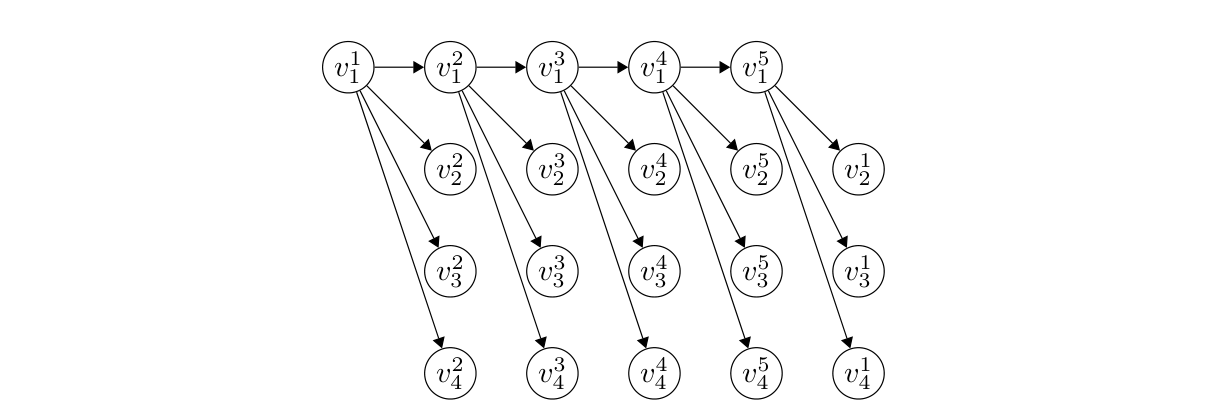
\includegraphics[width=\linewidth]{trace-fig1.png}\caption{The spanning tree construction for width 4 and $d=5$.}\end{figure}
\begin{figure}[tbp]\centering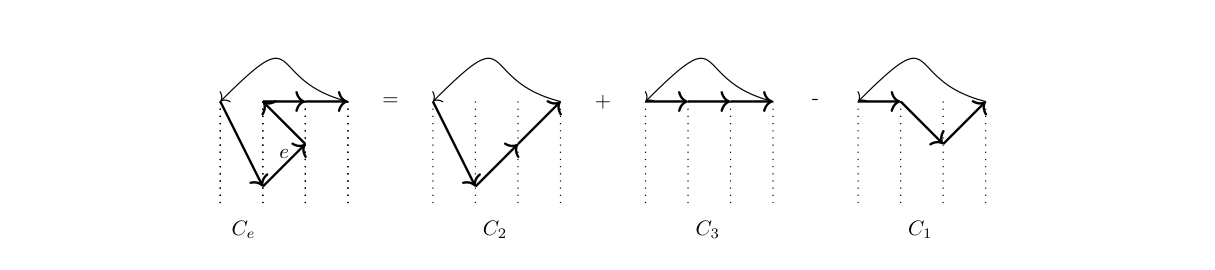
\includegraphics[width=\linewidth]{trace-fig2.png}\caption{Decomposing a cycle of length $d+2$ as a linear combination of cycles of length $d$. The figure is an illustration when $d=3$. The dotted layers in each cycle from the left are $V^3$, $V^1$, $V^2$, and $V^3$ again.}\end{figure}
\begin{proof}
We construct a spanning tree $\tau$ as follows, which will be a tree whose edges are all directed away from its root. Informally, the tree is given by the following subgraph, we make the first vertex in $V^1$ as root, and include all the outgoing edges incident to it. We then move to the first vertex in $V^2$ and include all the outgoing edges incident to it. We continue in this way until we reach $V^d$. Upon reaching the first vertex in $V^d$ we include all but one outgoing edges incident to it. The one that is an incoming edge to the root is not included. Figure 1 illustrates the construction. We now formally define this.
Let $v^i_1\in V^i$ denote the first vertex in the layer $i$, $1\le i\le d$. Further recall $\inset(v)\subseteq E$ and $\outset(v)\subseteq E$ denote the set of incoming and outgoing edges, respectively, incident to $v$. Define the edge set
\[\tau:=\left(\bigcup_{i=1}^d\outset(v^i_1)\right)\setminus\{(v^d_1,v^1_1)\},\]
which is a spanning tree in $\widetilde\Gamma$. We know that every edge not in the tree when added to the tree gives a unique undirected cycle. We now show that the characteristic flows of these undirected cycles can be expressed as a linear combination of the characteristic flows of directed cycles of length $d$. For $e\in E\setminus\tau$, let $c_e$ denote the characteristic flow of the unique undirected cycle that uses $e$ in its correct direction and only edges of $\tau$. We argue depending on which layer the edge $e$ belongs to.
\paragraph{Suppose $e\in E^1\setminus\tau$.}
\begin{itemize}
\item If $e$ is incident to $v^2_1$, the first vertex in $V^2$, then the inclusion of $e$ creates a directed cycle of length $d$. Hence, $c_e$ equals the characteristic flow of this directed cycle.
\item Otherwise, the inclusion of $e$ creates an undirected cycle of length $d+2$. If $e=(v^1_{j_1},v^2_{j_2})$ for some $j_1\in[2,w_1]$ and $j_2\in[2,w_2]$, then the cycle $c_e$ is given as follows:
\[v^d_1-v^1_{j_1}-v^2_{j_2}-v^1_1-v^2_1-\cdots-v^{d-1}_1-v^d_1.\]
Consider the following two directed cycles:
\begin{align*}C_1&:v^1_1-v^2_{j_2}-\cdots-v^d_1-v^1_1\text{ and}\\C_2&:v^1_{j_1}-v^2_{j_2}-\cdots-v^d_1-v^1_{j_1},\end{align*}
such that the part $v^2_{j_2}-\cdots-v^d_1$ between $v^2_{j_2}$ and $v^d_1$ in the two cycles is the same. Let us denote the characteristic flow of a cycle $C$ by $\chi(C)$. We now observe that $\chi(C_2)-\chi(C_1)$ equals the characteristic flow of the undirected cycle $v^1_{j_1}-v^2_{j_2}-v^1_1-v^d_1-v^1_{j_1}$. This is because the common part in $C_1$ and $C_2$ cancels out. To $\chi(C_2)-\chi(C_1)$ we add the characteristic flow of the directed cycle,
\[C_3:v^1_1-v^2_1-v^3_1-\cdots-v^{d-1}_1-v^d_1-v^1_1.\]
It is now easily seen that $\chi(C_2)-\chi(C_1)+\chi(C_3)$ equals the characteristic flow of the cycle $c_e$ (see Figure 2 for an illustration).
\end{itemize}
\paragraph{Suppose $e\in E^d\setminus\tau$.}
\begin{itemize}
\item If $e$ is incident to $v^1_1$, the first vertex in $V^1$, then as before the inclusion of $e$ creates a directed cycle of length $d$. Hence, $c_e$ equals the characteristic flow of this directed cycle.
\item Otherwise, the inclusion of $e$ creates an undirected cycle of length4. If $e=(v^d_{j_1},v^1_{j_2})$ for some $j_1\in[2,w_d]$ and $j_2\in[2,w_1]$, then the cycle $c_e$ is given as follows:
\[v^d_{j_1}-v^1_{j_2}-v^d_1-v^{d-1}_1-v^d_{j_1}.\]
Consider the following two directed cycles:
\begin{align*}C_4&:v^1_{j_2}-\cdots-v^{d-1}_1-v^d_1-v^1_{j_2}\text{ and}\\C_5&:v^1_{j_2}-\cdots-v^{d-1}_1-v^d_{j_1}-v^1_{j_2},\end{align*}
such that the part $v^1_{j_2}-\cdots-v^{d-1}_1$ between $v^1_{j_2}$ and $v^{d-1}_1$ in the two cycles is the same. We now claim that $\chi(C_5)-\chi(C_4)$ equals the characteristic flow of $c_e$. This is because the common part in $C_4$ and $C_5$ cancels out.
\end{itemize}
Otherwise $e\in E^i\setminus\tau$ for some $i\in\{2,\ldots,d-1\}$. In such a case inclusion of $e$ creates an undirected cycle of length4. We can again argue exactly like in the previous case, and so we omit the argument here.
\end{proof}
We now prove that the generating set given by the directed cycles of length $d$ is contained in the image of $T$ under the map $\varrho$.
\begin{claim}$\im(\varrho|_T)$ contains the characteristic flow of each directed cycle of length $d$.\end{claim}
\begin{proof}
Let $\{e_1,e_2,\ldots,e_d\}\subseteq E$ be a directed cycle of length $d$, where each $e_i$ points from a vertex in $V^i$ to a vertex in $V^{i+1}$. Let $\{e_i^{(j)}\}$ denote the set of edges that start at the same vertex as $e_i$, but for which $e_i^{(j)}\ne e_i$. Thus $|\{e_i^{(j)}\}|=|V^{i+1}|-1$. Let
\[\bar\psi(e):=\frac1{|\{p\in\mathcal P\text{ with }e\in p\}|}\psi(e),\]
so that $\varrho(\bar\psi(e))$ is a flow with value 1 on the edge $e$. It is instructive to have a look at the left side of Figure 3, where $\varrho(\bar\psi(e_1))$ is depicted. Subtracting $\frac1{w_3}\sum_{j=1}^{w_3-1}\varrho(\bar\psi(e_2^{(j)}))$ and adding $\frac{w_3-1}{w_3}\varrho(\bar\psi(e_2))$ reduces the support significantly and brings us one step closer to the cycle, see the right side of Figure 3. We iterate this process until only the cycle is left. Formally:
\begin{align*}
\chi(e_1,\ldots,e_d)={}&\varrho(\bar\psi(e_1))\\
&+\frac{w_3-1}{w_3}\varrho(\bar\psi(e_2))-\frac1{w_3}\sum_{j=1}^{w_3-1}\varrho(\bar\psi(e_2^{(j)}))\\
&+\cdots\\
&+\frac{w_d-1}{w_d}\varrho(\bar\psi(e_{d-1}))-\frac1{w_d}\sum_{j=1}^{w_d-1}\varrho(\bar\psi(e_{d-1}^{(j)})).
\end{align*}
\end{proof}
\begin{figure}[tbp]\centering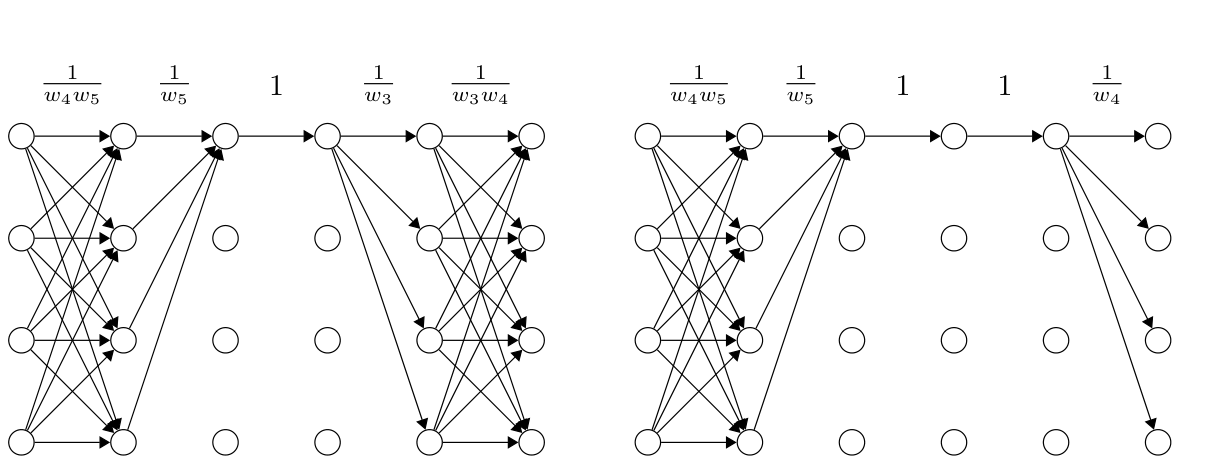
\includegraphics[width=\linewidth]{trace-fig3.png}\caption{On the left: $\varrho(\bar\psi(e_1))$. On the right: $\varrho(\bar\psi(e_1))-\frac1{w_3}\sum_{j=1}^{w_3-1}\varrho(\bar\psi(e_2^{(j)}))+\frac{w_3-1}{w_3}\varrho(\bar\psi(e_2))$. This is the case $d=5$ and format$(4,4,4,4,4)$. Edges that are not drawn carry 0 flow. All edges in the same layer carry either0 flow or the value that is depicted above the edge layer. For the purposes of illustation, $e_1$ is the top edge in the center. Here we assume that each $e_i$ points from the first vertex in $V^i$ to the first vertex in $V^{i+1}$.}\end{figure}
\paragraph{The stronger upper bound via parities.}
We now proceed to upper bound $\dim T'$ (Theorem 14). The proof is analogous to the proof of Lemma 15.
\begin{theorem}[Restatement of Theorem 14]$\dim T'\le|E|-|\widetilde V|$.\end{theorem}
\begin{proof}
As in the proof of Lemma 15, for $v\in\widetilde V$, we have
\[\sum_{e\in\inset(v)}\psi'(e)=\sum_{e\in\outset(v)}\psi'(e).\]
Furthermore, we have the following additional constraint on $\psi'$,
\[(d-1)\sum_{e\text{ parity preserving}}\psi'(e)=\sum_{e\text{ parity changing}}\psi'(e).\]
By the linearity of $\psi'$, we have
\[\psi'\left((d-1)\sum_{e\text{ parity preserving}}\chi(e)-\sum_{e\text{ parity changing}}\chi(e)\right)=0.\]
Therefore, the kernel of $\psi'$ is spanned by the vectors $(\sum_{e\in\inset(v)}\chi(e)-\sum_{e\in\outset(v)}\chi(e))$, for $v\in\widetilde V$, and an additional vector $((d-1)\sum_{e\text{ parity preserving}}\chi(e)-\sum_{e\text{ parity changing}}\chi(e))$.
We now claim that the new vector is linearly independent from the earlier set of vectors. We prove the claim by constructing a vector in $\C^E$ that is orthogonal to the earlier set of vectors but is non-orthogonal to the additional vector. One such vector is given by the characteristic flow of the directed cycle $v^1_1-v^2_1-v^3_1-\cdots-v^{d-1}_1-v^d_1-v^1_1$.
Thus, it follows that $\dim\ker\psi'\ge|\widetilde V|$, and hence $\dim T'\le|E|-|\widetilde V|$.
\end{proof}

\begin{thebibliography}{42}
\bibitem{ref1} Eric Allender and Fengming Wang. On the power of algebraic branching programs of width two. Comput. Complex., 25(1):217–253, March 2016. doi:10.1007/s00037-015-0114-7.
\bibitem{ref2} Jarod Alper, Tristram Bogart, and Mauricio Velasco. A lower bound for the determinantal complexity of a hypersurface. Foundations of Computational Mathematics, pages 1–8, 2015.
\bibitem{ref3} Matthew Anderson, Michael A. Forbes, Ramprasad Saptharishi, Amir Shpilka, and Ben Lee Volk. Identity testing and lower bounds for read-k oblivious algebraic branching programs. In Proceedings of the 31st Conference on Computational Complexity, CCC ’16, Dagstuhl, DEU, 2016. Schloss Dagstuhl–Leibniz-Zentrum fuer Informatik.
\bibitem{ref4} Michael Ben-Or and Richard Cleve. Computing algebraic formulas using a constant number of registers. SIAM J. Comput., 21(1):54–58, 1992. doi:10.1137/0221006.
\bibitem{ref5} D. Bini. Relations between exact and approximate bilinear algorithms. applications. CALCOLO, 17(1):87–97, January 1980. doi:10.1007/BF02575865.
\bibitem{ref6} Dario Bini, Milvio Capovani, Francesco Romani, and Grazia Lotti. O(n2.7799) complexity for n × n approximate matrix multiplication. Inf. Process. Lett., 8(5):234–235, 1979. doi: 10.1016/0020-0190(79)90113-3.
\bibitem{ref7} Markus Bläser and Christian Ikenmeyer. Introduction to geometric complexity theory, 2018. , version from July 25. URL: http://pcwww.liv.ac.uk/~iken/teaching\_sb/summer17/ introtogct/gct.pdf.
\bibitem{ref8} J.A. Bondy and U.S.R Murty. Graph Theory. Springer Publishing Company, Incorporated, 2008.
\bibitem{ref9} Karl Bringmann, Christian Ikenmeyer, and Jeroen Zuiddam. On algebraic branching programs of small width. J. ACM, 65(5), August 2018. doi:10.1145/3209663.
\bibitem{ref10} Peter Bürgisser. Erratum to the complexity of factors of multivariate polynomials. URL: https://www.math.tu-berlin.de/fileadmin/i26\_fg-buergisser/erratum\_factors.pdf.
\bibitem{ref11} Peter Bürgisser. Completeness and Reduction in Algebraic Complexity Theory. Springer Berlin Heidelberg, Berlin, Heidelberg, 2000.
\bibitem{ref12} Peter Bürgisser. The complexity of factors of multivariate polynomials. Found. Comput. Math., 4(4):369–396, 2004. doi:10.1007/s10208-002-0059-5.
\bibitem{ref13} Peter Bürgisser, Michael Clausen, and Mohammad A Shokrollahi. Algebraic complexity theory, volume 315. Springer Science \& Business Media, 2013.
\bibitem{ref14} Peter Bürgisser, J.M. Landsberg, Laurent Manivel, and Jerzy Weyman. An overview of mathematical issues arising in the Geometric complexity theory approach to VP v.s. VNP. SIAM J. Comput., 40(4):1179–1209, 2011.
\bibitem{ref15} Prerona Chatterjee, Mrinal Kumar, Adrian She, and Ben Lee Volk. A quadratic lower bound for algebraic branching programs. CoRR, abs/1911.11793, 2019. To appear in the proceedings of Conference on Computational Complexity, CCC’20. arXiv:1911.11793.
\bibitem{ref16} Michael Forbes. Some concrete questions on the Border Complexity of polynomials, 2016. Talk at the Workshop on Algebraic Complexity Theory (WACT) 2016 in Tel Aviv. URL: https://www.youtube.com/watch?v=1HMogQIHT6Q.
\bibitem{ref17} Hervé Fournier, Guillaume Malod, Maud Szusterman, and Sébastien Tavenas. Nonnegative rank measures and monotone algebraic branching programs. In 39th IARCS Annual Conference on Foundations of Software Technology and Theoretical Computer Science, volume 150 of LIPIcs. Leibniz Int. Proc. Inform., pages Art. No. 15, 14. Schloss Dagstuhl. Leibniz-Zent. Inform., Wadern, 2019.
\bibitem{ref18} Fulvio Gesmundo. Geometric aspects of iterated matrix multiplication. Journal of Algebra, 461:42–64, 2016.
\bibitem{ref19} Fulvio Gesmundo, Christian Ikenmeyer, and Greta Panova. Geometric complexity theory and matrix powering. Differential Geom. Appl., 55:106–127, 2017. doi:10.1016/j.difgeo.2017. 07.001.
\bibitem{ref20} Bruno Grenet. An upper bound for the permanent versus determinant problem, 2011. Manu- script. URL: http://www.lirmm.fr/~grenet/publis/Gre11.pdf.
\bibitem{ref21} Joshua A. Grochow, Ketan D. Mulmuley, and Youming Qiao. Boundaries of VP and VNP. In 43rd International Colloquium on Automata, Languages, and Programming, volume 55 of LIPIcs. Leibniz Int. Proc. Inform., pages Art. No. 34, 14. Schloss Dagstuhl. Leibniz-Zent. Inform., Wadern, 2016.
\bibitem{ref22} Joos Heintz and Malte Sieveking. Lower bounds for polynomials with algebraic coefficients. Theoretical Computer Science, 11(3):321–330, 1980.
\bibitem{ref23} Jesko Hüttenhain. Geometric Complexity Theory and Orbit Closures of Homogeneous Forms. PhD thesis, Technische Universität Berlin, July 2017.
\bibitem{ref24} Jesko Hüttenhain and Pierre Lairez. The boundary of the orbit of the 3-by-3 determinant polynomial. Comptes Rendus Mathematique, 354(9):931–935, 2016.
\bibitem{ref25} Neeraj Kayal, Vineet Nair, Chandan Saha, and Sébastien Tavenas. Reconstruction of full rank algebraic branching programs. ACM Trans. Comput. Theory, 11(1), November 2018. doi:10.1145/3282427.
\bibitem{ref26} Mrinal Kumar. On top fan-in vs formal degree for depth-3 arithmetic circuits, 2018. URL: https://eccc.weizmann.ac.il/report/2018/068/.
\bibitem{ref27} Mrinal Kumar. A quadratic lower bound for homogeneous algebraic branching programs. computational complexity, 28(3):409–435, 2019. doi:10.1007/s00037-019-00186-3.
\bibitem{ref28} J. M. Landsberg. Geometric complexity theory: an introduction for geometers. ANNALI DELL’UNIVERSITA’ DI FERRARA, 61(1):65–117, May 2015.
\bibitem{ref29} J. M. Landsberg. Geometry and Complexity Theory. Cambridge Studies in Advanced Math- ematics. Cambridge University Press, 2017. doi:10.1017/9781108183192.
\bibitem{ref30} Meena Mahajan and V. Vinay. Determinant: combinatorics, algorithms, and complexity. Chicago J. Theoret. Comput. Sci., pages Article 5, 26 pp. (electronic), 1997.
\bibitem{ref31} Guillaume Malod and Natacha Portier. Characterizing Valiant’s algebraic complexity classes. Journal of Complexity, 24(1):16–38, 2008.
\bibitem{ref32} K.D. Mulmuley and M. Sohoni. Geometric Complexity Theory. I. An approach to the P vs. NP and related problems. SIAM J. Comput., 31(2):496–526 (electronic), 2001.
\bibitem{ref33} K.D. Mulmuley and M. Sohoni. Geometric Complexity Theory. II. Towards explicit obstructions for embeddings among class varieties. SIAM J. Comput., 38(3):1175–1206, 2008.
\bibitem{ref34} D. Mumford. Algebraic geometry. I: Complex projective varieties. Classics in mathematics. Springer-Verlag, Berlin, 1995. Reprint of the 1976 edition in Grundlehren der mathematischen Wissenschaften, vol. 221.
\bibitem{ref35} Noam Nisan. Lower bounds for non-commutative computation. In Proceedings of the twenty- third annual ACM symposium on Theory of computing, pages 410–418. ACM, 1991.
\bibitem{ref36} Ran Raz. Tensor-rank and lower bounds for arithmetic formulas. J. ACM, 60(6):Art. 40, 15, 2013. doi:10.1145/2535928.
\bibitem{ref37} Claus-Peter Schnorr. Improved lower bounds on the number of multiplications/divisions which are necessary to evaluate polynomials. In International Symposium on Mathematical Foundations of Computer Science, pages 135–147. Springer, 1977.
\bibitem{ref38} Srikanth Srinivasan. Strongly exponential separation between monotone VP and monotone VNP, 2019. arXiv:1903.01630.
\bibitem{ref39} Volker Strassen. Polynomials with rational coefficients which are hard to compute. SIAM Journal on Computing, 3(2):128–149, 1974.
\bibitem{ref40} Seinosuke Toda. Classes of Arithmetic Circuits Capturing the Complexity of the Determinant. IEICE TRANS. INF. \& SYST., E75-D(1):116–124, 1992.
\bibitem{ref41} L. G. Valiant. Completeness classes in algebra. In Conference Record of the Eleventh Annual ACM Symposium on Theory of Computing (Atlanta, Ga., 1979), pages 249–261. ACM, New York, 1979.
\bibitem{ref42} Amir Yehudayoff. Separating monotone VP and VNP. In Proceedings of the 51st Annual ACM SIGACT Symposium on Theory of Computing, STOC 2019, page 425–429, New York, NY, USA, 2019. Association for Computing Machinery. doi:10.1145/3313276.3316311.
\end{thebibliography}
\end{document}
